\documentclass[main.tex]{subfiles}
\begin{document}
\section{Parametric and Line Spectra}

Non-Parametric spectral estimation methods are general approaches to finding frequency components of a real-world signal. However, certain properties of our signal are known to us. This invaluable information can be used in different parametric spectral estimation methods to improve the performance.


%%%%%%%%%%%%%%%%%%%%%%%%%%%%%%%%%%%%%%%%%%%%%%%%%%%%%%%%%%%%
%%%%%%%%%%%%%%%%%%%%%%%%%%%%%%%%%%%%%%%%%%%%%%%%%%%%%%%%%%%%
%%%%%%%%%%%%%%%%%%%%%%%%%%%%%% 2.1
%%%%%%%%%%%%%%%%%%%%%%%%%%%%%%%%%%%%%%%%%%%%%%%%%%%%%%%%%%%%
%%%%%%%%%%%%%%%%%%%%%%%%%%%%%%%%%%%%%%%%%%%%%%%%%%%%%%%%%%%%
\subsection{Correlation Estimation}

Recall that that the Discrete Fourier Transform (DFT) of the auto-correlation of a signal is equivalent to the PSD of that same signal, such that

\begin{equation}
P(\omega) = \sum_{k=-(k-1)}^{N-1}\hat{r}e^{jwk}
\end{equation}

where the autocorrelation is estimated based on the available samples. Following from the definition of the autocorrelation, an appropriate estimating equation could be \ref{eq:2-1-1-ub}. Immediately a problem arises; calculating the autocorrelation for large values of $k$ will have many less reference points than for low $k$.  As there are fewer samples, the estimate at large values of $k$ can be  erratic; which in turn may make result in a non-positive definite ACF, resulting in a negative PSD.


\begin{align}
\text{Unbiased: } \hat{r}(k) &= \frac{1}{N-k}\sum_{n=k+1}^{N}x(n)x^*(n-k) \label{eq:2-1-1-ub}\\
\text{Biased: } \hat{r}(k) &= \frac{1}{N}\sum_{n=k+1}^{N}x(n)x^*(n-k) \label{eq:2-1-1-b}
\end{align}


The biased estimator (eq \ref{eq:2-1-1-b}) solves this issue, but introduces a distortion to the ACF as a function of k. This effect can be seen in figure~\ref{fig:2-1-a-vs} (\textit{The theoretical ACF of a WGN-corrupted sinusoid should be a sinusoid with a positive offset of $\sigma_{\eta}^2$}).

\begin{figure}[H]
	\centering 
	\resizebox{\textwidth}{!}{\input{matlabimages/2-1-a-vs.tikz}}
	\caption{Biased against unbiased ACF estimators. Note how at large lag, the ubiased esimator gives erratic results, even though the general shape of the unbiased ACF more closely resembles the ideal ACF. }
	\label{fig:2-1-a-vs}
\end{figure}

\subsubsection{Estimating the PSD using Biased and Unbiased Estimators}

To investigate the effects of the biased and unbiased ACF estimators, three signals are generated and the PSD calculated using both equations \ref{eq:2-1-1-ub} and \ref{eq:2-1-1-b} with $P(\omega) = F(r(k))$. The results, are shown in figure~\ref{fig:q2_1_a}.

\begin{figure}[H]
	\centering 
	\resizebox{\textwidth}{!}{\input{matlabimages/2-1-a.tikz}}
	\caption{}
	\label{fig:q2_1_a}
\end{figure}

It's important to note that the unbiased ACF is erradic at high values of $k$, and therefore is not positive definite. This causes negative points on the PSD, which are conceptually impossible. 





\subsubsection{Estimating the PSD}

In figure~\ref{fig:2-1-b}, 20 realisations of 2 sinusoids corrupted by WGN are shown in cyan ($F_s = 300Hz$, $f_1= 30Hz$, $f_2=50Hz$). The mean is superposed in blue. 

As expected, the PSD shows two clear spikes at 0.2 ($30/150$) and 0.33 ($50/150$)$\pi rads$. From the standard deviation of the PSD, it's relevant to note that, again, two peaks happen around 0.2 and 0.33. This comes from the fact that each realisation spikes a different amount in this region, therefore the variance is large. Outside the two spikes around $f_1$ and $f_2$, the realisations are very close to 0, thus the variance is close to 0.

\begin{figure}[H]
	\centering
	\begin{subfigure}[b]{0.9\textwidth}
		\resizebox{\textwidth}{!}{\input{matlabimages/2-1-b-a.tikz}}
		\label{fig:2-1-b-a}
	\end{subfigure}%
	
	\begin{subfigure}[b]{0.9\textwidth}
		\resizebox{\textwidth}{!}{\input{matlabimages/2-1-b-b.tikz}}
		\label{fig:2-1-b-b}
	\end{subfigure}
	\caption{Scalar (left) and Logarithmic (Right) representation of PSD using ensamble mean and variance.}
	\label{fig:2-1-b}
\end{figure}


\subsubsection{Estimating the PSD (logarithmic analysis)}


The same analysis as above is made while looking at logarithmic scales. As the logarithm accentuates only the changes in the signal, two important factors change when compared to the scalar axis;

\begin{itemize}
	\item \textbf{The variation of noise is significantly higher.} This comes from the fact that small fluctuations in noise around 0 now become relevant.
	\item \textbf{The variation around the peaks is significantly lower.} Again, as changes are accentuated in log, the variance around $f_1$ and $f_2$ significantly reduces. As each instansisation will spike significantly at these two points, the actual value it jumps to is unimportant; what matters is the order of magnitude by which it increases (Order 10).
\end{itemize}

\paragraph{Looking at the PSD estimate in logarithmic scales} is benefitial as it allows for easier identification of spikes, even with a small number of instantiasations.

\subsubsection{Generation of Complex Signals}

It is generally useful to consider complex signals. This is particularly true in communications, and 2-dimensional environment information (such as wind data). To this purpose, the concept of complex signals corrupted by complex (and circular) WGN and their PSDs are introduced.

Complex signals are gnerally generated using a complex exponent. In figure~\ref{fig:q2_1_d}, the pure signal is defined by

\[
x = e^{1j2\pi 0.3\textbf{n}} + exp^{1j2\pi 0.32\textbf{n}}
\]

Complex, circular\footnote{Circular complex WGN has mean 0 and equal variance in all direction (i.e. probability space is defined by a perfect gaussian plane in the complex space that is centered at 0)} WGN can be generated in Matlab with

\begin{lstlisting}[frame=single]
std_dev = 0.2;
noise = std_dev * 1/sqrt(2) * ([1 1j] * randn([2 length(n)]));
\end{lstlisting}

\paragraph{When considering the PGM-PSD estimated, } it's important to note that the number of samples used are vital for frequency resolution. As shown in fig~\ref{fig:q2_1_d}, if the sample size is too small, it becomes impossible to identify nearby-frequency peaks. 

\begin{figure}[H]
	\centering 
	\resizebox{\textwidth}{!}{\input{matlabimages/2-1-d.tikz}}
	\caption{Periodogram Power Spectral Density estimate for complex signals with a varying number of samples. As the number of samples increase from 30 to 60, the resolution increases and identification of the spikes at 0.3 and 0.32 can be more easily identified}
	\label{fig:q2_1_d}
\end{figure}


\subsubsection{Multiple Signal Classification Algorithm (MUSIC)}

The main concept behind the MUltiple SIgnal Classification (MUSIC) algorithm, is to decompose the autocorrelation matrix into it's constituant eigen vector/value pairs. These are then used to classify each frequency as noise or signal. From here, a pseudospectrum that resembles the underlying noise-free PSD can be drawn.

Assume a given signal $\textbf{x}$ is driven by $\textbf{p}$ complex exponentials in complex, circular WGN. The eigenvectors corresponding to the $p$ largest eigenvalues will hold the (\textit{noise-free}) signal span space. The remaining $M-p$ eigenvectors hold only noise. 

The psudospectrum can then be plotted as

\[
\hat P_{MU}(e^{j \omega}) = \frac{1}{\sum_{i=p+1}^{M} |\mathbf{e}^{H} \mathbf{v}_i|^2}
\]

Using the provided code, the results are shown in figure~\ref{fig:q2_1_e}.

\begin{figure}[H]
	\centering 
	\resizebox{\textwidth}{!}{\input{matlabimages/2-1-e.tikz}}
	\caption{}
	\label{fig:q2_1_e}
\end{figure}

\paragraph{Matlab Implementation}

\begin{itemize}
	\item {\tt [X,R] = corrmtx(x,14,'mod')}
	
	This calculated the Toepliz matrix $\textbf{X} \in R^{(n+m)x(m+1)}$ , which can be used to generate the autocorrelation matrix of the input. Inputs are {\tt x}, the data on which to apply MUSIC. The second argument defined {\tt mod} is used to explain the format of the output (in this case the m*m autocorrelation of M).
	
	The outputs are {\tt X}, the Toeplitz matrix and {\tt R}, the autocorrelation matrix.
	\item {\tt [S,F] = pmusic(R,2,[ ],1,'corr')}
	
	This calculated the pseudospectrum using the MUSIC algorithm. The inputs are (sequentially) the autocorrelation matrix calculated above, the dimension of the signal subspace (\textit{how many complex signals}), the length of the fft (nfft), 'corr' to specify the first input was the correlation matrix.
	
	The output is S, the pseudospectrum calculated by the MUSIC algorithm, and F, the relevant frequencies.
	\item {\tt plot(F,S,'linewidth',2); set(gca,'xlim',[0.25 0.40]) }
	
	This will plot the MUSIC pseudospectrum with a line thickness of 2, and focus on the frequencies between 0.25 and 0.4.
\end{itemize}

\paragraph{Advantages of the MUSIC.}

With enough information about the underlying algorithm, MUSIC is able to almost perfectly generate a PSD. It requires very few data points, and is able to generate perfectly smooth spectral density plots. Furthermore, as the output is continuously calculated, there are no issues around frequency resolution as in other estimation methods.

\paragraph{Disadvantages of MUSIC.} As mention above, the MUSIC algorithm is able to perform outstandingly, but only when enough data about the underlying signal is known. As expained by the parameters above, one must know the number of underlying complex signals. Without this information, the pseudospectrum generated by the MUSIC algorithm may be misleading or incorrect.



%%%%%%%%%%%%%%%%%%%%%%%%%%%%%%%%%%%%%%%%%%%%%%%%%%%%%%%%%%%%
%%%%%%%%%%%%%%%%%%%%%%%%%%%%%%%%%%%%%%%%%%%%%%%%%%%%%%%%%%%%
%%%%%%%%%%%%%%%%%%%%%%%%%%%%%% 2.2
%%%%%%%%%%%%%%%%%%%%%%%%%%%%%%%%%%%%%%%%%%%%%%%%%%%%%%%%%%%%
%%%%%%%%%%%%%%%%%%%%%%%%%%%%%%%%%%%%%%%%%%%%%%%%%%%%%%%%%%%%
\subsection{Spectrum of Autoregressive Processes}


\subsubsection{Shortcomings of the unbiased ACF estimate}

Although the unbiased ACF more closely resembles the theoretical ACF, it was shown in 2.1 to have erratic values for large time lags ($k$). This means the matrix is non-positive definite, which results in it being non-invertible. 

This is a significant problem when trying to estimate the parameters for an AR process, as $\textbf{a} = \ref{fig:q2_1_d}_{xx}^{-1}\textbf{R}_{xx}$.

Furthermore, even if $\textbf{R}_{xx}$ is invertible, the erratic nature at high lags will give large values - and therefore incorrect values for $\textbf{a}$.

\subsubsection{Estimation of PSD}

As the unbiased estimator will lead to problems when trying to estimate the AR coefficients, the biased estimator is used to find $\textbf{a}$. With these values, the PSD can be plotted, as shown in figure~\ref{fig:q2_3_b} for the AR process

\[
x(n) = 2.76x(n-1) - 3.81x(n-2) +2.65x(n-1) -0.92x(n-4) + w(n)
\]

\begin{figure}[H]
	\centering 
	\resizebox{\textwidth}{!}{\input{matlabimages/2-2-b.tikz}}
	\caption{PSD estimate using AR(M) coefficient method using 1,000 estimates. Order of 2, 4 and 14 are trialled}
	\label{fig:q2_3_b}
\end{figure}

Through experimentation, it is shown that the model order equal to that of the original AR process is ideal for calculating the PSD. This can be seen in figure~\ref{fig:q2_3_b} as the PSD holds much the same shape between $AR(5)$ and $AR(14)$. 




\subsubsection{Effect of Model Order on PSD Estimate}

\paragraph{By under-modelling the AR-process}, the PSD estimate hold an incorrect shape, and does not show peaks at the correct frequency. As this is incorrect, the effect of under-modelling is to render the PSD estimate inaccurate.

\paragraph{Although over-modelling increases the quality (resolution) of the PSD,} it's important to note that this comes at a significanly increased computational load. As such, it's not recommended to unneccesarily increase the model order.

\begin{figure}[H]
	\centering 
	\resizebox{\textwidth}{!}{\input{matlabimages/2-2-c.tikz}}
	\caption{Reptition of experiment from figure~\ref{fig:q2_3_b}, but with 10,000 samples}
	\label{fig:q2_3_c}
\end{figure}


In result, a cost-benefit analysis of resolution vs. computational complexity must be considered when deciding the model order. In situations where the model order is know to be $M$, it is recommended to hold the model order between $M$ and $M+2$, as beyond this the benefits to the PSD are unneccessarily.






%%%%%%%%%%%%%%%%%%%%%%%%%%%%%%%%%%%%%%%%%%%%%%%%%%%%%%%%%%%%
%%%%%%%%%%%%%%%%%%%%%%%%%%%%%%%%%%%%%%%%%%%%%%%%%%%%%%%%%%%%
%%%%%%%%%%%%%%%%%%%%%%%%%%%%%% 2.3
%%%%%%%%%%%%%%%%%%%%%%%%%%%%%%%%%%%%%%%%%%%%%%%%%%%%%%%%%%%%
%%%%%%%%%%%%%%%%%%%%%%%%%%%%%%%%%%%%%%%%%%%%%%%%%%%%%%%%%%%%
\subsection{Time-Frequency Estimation}

\subsubsection{Introduction of {\tt spectrogram}}

To investigate the properties of the {\tt spectrogram} function, a number of tests were run to determine the effects of $window, noverlap, nfft$, and $fs$ on the resulting spectrogram. (\textit{Through out the tests, the size of $window$ and $nfft$ were keps equal.})

\begin{figure}[H]
	\centering
	\begin{subfigure}[b]{\textwidth}
		\centering
		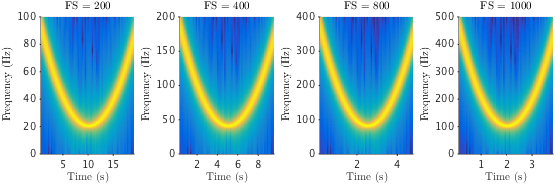
\includegraphics[width=0.8\textwidth]{images/2-3-a-1.png}
		\caption{Effect of {\tt fs} on the spectrogram. $fs=1000$ is clearly the only correct answer!}
		\label{fig:2-3-a-1}
	\end{subfigure}%
	
	\begin{subfigure}[b]{\textwidth}
		\centering
		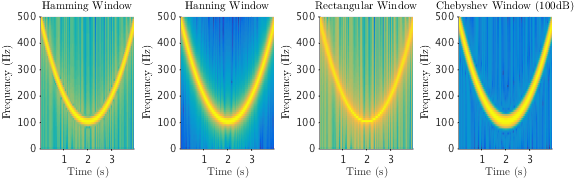
\includegraphics[width=0.8\textwidth]{images/2-3-a-2.png}
		\caption{Effect of {\tt window} type on the spectrogram.}
		\label{fig:2-3-a-2}
	\end{subfigure}
	
	\begin{subfigure}[b]{\textwidth}
		\centering
		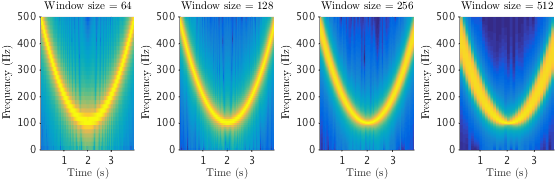
\includegraphics[width=0.8\textwidth]{images/2-3-a-3.png}
		\caption{Effect of {\tt nfft} and therefore the window size on the spectrogram.}
		\label{fig:2-3-a-3}
	\end{subfigure}
	
	\begin{subfigure}[b]{\textwidth}
		\centering
		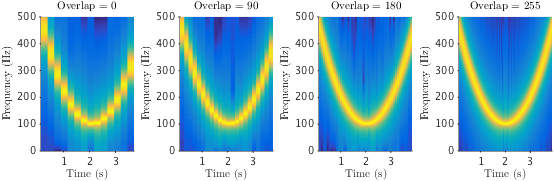
\includegraphics[width=0.8\textwidth]{images/2-3-a-4.png}
		\caption{Effect of {\tt noverlap} on the spectrogram.}
		\label{fig:2-3-a-4}
	\end{subfigure}
	\caption{Experimenting with {\tt spectrogram}}
	\label{fig:2-3-a}
\end{figure}


The results gathered from experimentation; (some of these tests shown in figure~\ref{fig:2-3-a})

\begin{enumerate}
	\item \textbf{\textit{fs}} is the sampling frequency. The spectrogram uses this to scale the x-axis (from 0 to length(x)/fs seconds) and the y-axis (0 to fs/2 Hz). 
	
	From the {\tt chirp} function, the sampling frequency is extracted as 1000. 
	
	\item \textbf{\textit{window}} defined the window to be used. The Hamming, Hanning, Rectangular and Chebyshev windows were tested.
	
	The Hanning window was chosen as it provided the largest deviation in the frequency domain. 
	
	\item \textbf{\textit{nfft}} was used as both the size of the window, but also as the resolution of the FFT inside the {\tt spectrogram} function. Increasing the FFT generally increases the resolution of the spectrogram in the y-axis, but at an additional computational cost.
	
	An FFT of around 128 or 256 was found to be ideal, as beyond this the hanning window spread the frequency domain too much.
	
	\item \textbf{\textit{noverlap}} defined the overlap between time windows. Increasing this value improved the time resolution, but at a significant cost to computation and memory (\textit{as there are many more values for the spectrogram!}).
	
	An overlap of around $80\%$ was found best in most analytical cases; however, it is worth dropping this to improve speed.
\end{enumerate}

\subsubsection{Time-Frequency analysis of EEG data}

Applying our learnings form the previous section to the EEG data from section 1.4 wil allow us to verify our previous findings. The EEG POz data is passed through the spectrogram function with a hanning window, 30\% overlap and nfft = $[2046, 4096]$, as these were shown to produce the best results.

\begin{figure}[H]
	\centering
	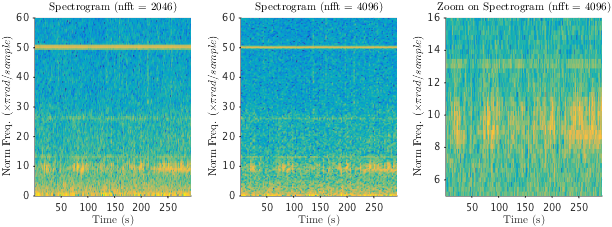
\includegraphics[width=0.8\textwidth]{images/2-3-b-1.png}
	\caption{Spectrogram of the POz EEG data. Note the AZ hum at 50Hz, as well as brainwaves from 8-10 Hz. A faint line can be seen around 13Hz and 26Hz, corresponding to the SSVP}
	\label{fig:2-3-b}
\end{figure}

The reason for using such a high NFFT was from the desire to have a high frequency resolution. With a sampling frequency of $1200Hz$, the setting the {\tt nfft} value to $2046$ gives about 2 bins per Hertz. This is increased to around 4 bins per Hertz, allowing for better identification of the 13Hz SSVP.


%%%%%%%%%%%%%%%%%%%%%%%%%%%%%%%%%%%%%%%%%%%%%%%%%%%%%%%%%%%%
%%%%%%%%%%%%%%%%%%%%%%%%%%%%%%%%%%%%%%%%%%%%%%%%%%%%%%%%%%%%
%%%%%%%%%%%%%%%%%%%%%%%%%%%%%% 2.4
%%%%%%%%%%%%%%%%%%%%%%%%%%%%%%%%%%%%%%%%%%%%%%%%%%%%%%%%%%%%
%%%%%%%%%%%%%%%%%%%%%%%%%%%%%%%%%%%%%%%%%%%%%%%%%%%%%%%%%%%%
\subsection{Real World Signals: Respiratory Sinus Arrhythmia from RR-Intervals}

\subsubsection{PSD of RRI data}

Using the raw ECG data, RR-information was extracted for three experiments - normal breathing, breathing at 50Hz and breathing at 15Hz. The original PSD, as well as averaged versions are shown below.

\begin{figure}[H]
	\centering
	
	\begin{subfigure}[b]{\textwidth}
		\centering
		\resizebox{\textwidth}{!}{\input{matlabimages/2-4-a-psd1.tikz}}
		\caption{PSD for Experiment 1 with different window sizes}
		\label{fig:2-4-a-psd1}
	\end{subfigure}%
	
	\begin{subfigure}[b]{\textwidth}
		\centering
		\resizebox{\textwidth}{!}{\input{matlabimages/2-4-a-psd2.tikz}}
		\caption{PSD for Experiment 2 with different window sizes}
		\label{fig:2-4-a-psd2}
	\end{subfigure}%
	
	\begin{subfigure}[b]{\textwidth}
		\centering
		\resizebox{\textwidth}{!}{\input{matlabimages/2-4-a-psd3.tikz}}
		\caption{PSD for Experiment 3 with different window sizes}
		\label{fig:2-4-a-psd3}
	\end{subfigure}%
\end{figure}


\subsubsection{Identifications of anomalee}

Although the peaks in the spectrum are not where expected, there are clear anomalies in the PSDs of each experiment which can be extrapolated. Experiment 2 shows a frequency component not seen in other experiemnt at $123Hz$. Experiment 3 shows an peak at around $30Hz$. 

\pagebreak
\end{document}